\section{Análisis del rendimiento}

Tras configurar el cluster,  se realizaron algunos experimentos con el fin de comprobar el funcionamiento correcto y realizar un análisis del rendimiento de las máquinas.

Para hacer pruebas, se utilizó un programa sencillo que calcula el valor de pi encontrado en un repositorio de github \cite{openmpirepo}. Este programa se utilizó simplemente para comprobar que todo funcionaba y familiarizarse con slurm. 

Después, para realizar un análisis de rendimiento, se utilizó NPB: un \emph{benchmark} perteneciente a la NASA, interesante especialmente porque las distintas pruebas de paralelización utilizan la memoria de distintas formas.

\subsection{Métricas}

El objetivo principal del análisis de rendimiento es conseguir los mejores resultados en el menor tiempo posible y consumiendo el menor número de recursos posible.
\vspace{2mm}

A la hora de determinar el rendimiento de una arquitectura paralela, es común medir la eficiencia mediante estas dos medidas \cite{parelismoyrendimiento}:
\vspace{2mm}

\begin{itemize}
\item \textbf{Tiempo de ejecución o respuesta} de una aplicación.

\item \textbf{Productividad} (\emph{throughput}), el número de aplicaciones que es capaz de procesar por unidad de tiempo.
\end{itemize}

\vspace{2mm}
Sin embargo, aunque ofrecen información útil, son medidas demasiado simples, por lo que se introducen otras métricas como el \emph{speedup}, la eficiencia, la utilización, la redundancia y la calidad del paralelismo.

\vspace{6mm}
\textbf{Aceleración}
\vspace{2mm}

El \emph{speedup} mide la relación entre el tiempo de ejecución de un algoritmo en paralelo con respecto a lo que tarda el mismo algoritmo en resolver el problema de forma secuencial.

\begin{equation*}
    S(n) = \frac{T(1)}{T(n)}
\end{equation*}

Generalmente, speedup tiene un valor entre 0 y p (número de procesadores), donde lo ideal sería que fuera igual a p (Figura \ref{speedup}). Sin embargo, también cabe la posibilidad que el valor sea mayor que p, causando así un speedup superlineal. Cuando esto ocurre, suele deberse a la gestión interna de la memoria en el caso del algoritmo paralelo, en el que cada procesador trabaja con menos datos que en el algoritmo secuencial.
\vspace{4mm}

\begin{figure}[htb]
   \centering
   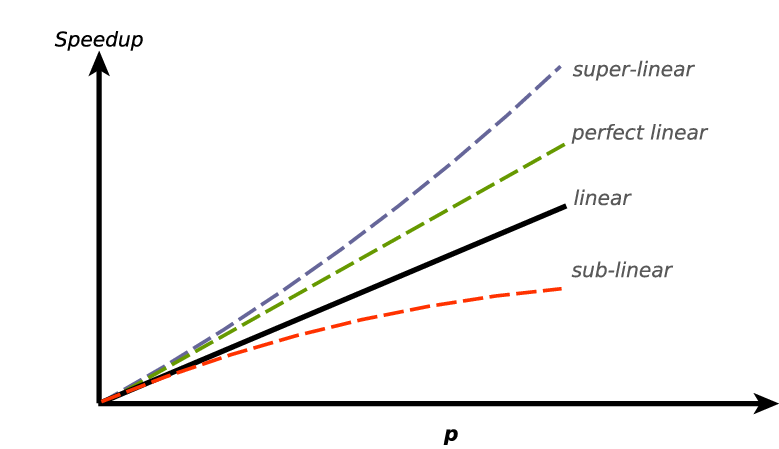
\includegraphics[scale=0.3]{images/speedup.png}
   \caption{SpeedUp}
   \label{speedup}
\end{figure}

\vspace{4mm}
\textbf{Eficiencia}
\vspace{2mm}

La eficiencia mide la fracción de tiempo durante la cual se utiliza de manera útil un procesador. Se obtiene dividiendo el speedup entre el número de procesadores.

\vspace{2mm}
\begin{equation*}
    E(n) = \frac{S(n)}{n} = \frac{T(1)}{n*T(n)}
\end{equation*}
\vspace{2mm}

Esta medida tendrá un valor entre 0 y 1, siendo 1 el valor ideal. Como ocurre con el speedup, también podemos obtener una eficiencia superior, si el speedup es superlineal.

\vspace{4mm}
\textbf{Redundancia}
\vspace{2mm}

La redundancia en un cálculo paralelo se define como el número total de operaciones ejecutadas con n procesadores dividido por el número de operaciones ejecutadas cuando utilizamos un único procesador.

\begin{equation*}
    R(n) = \frac{O(n)}{O(1)}
\end{equation*}

\vspace{4mm}
\textbf{Utilización}
\vspace{2mm}

La utilización de un sistema indica el porcentaje de recursos que se utilizan durante la ejecución de un programa paralelo.

\begin{equation*}
    U(n) = R(n)E(n) = \frac{O(n)}{n * T(n)}
\end{equation*}


\vspace{4mm}
\textbf{Calidad del paralelismo}
\vspace{2mm}

La calidad de un cálculo paralelo es directamente proporcional al speedup y la eficiencia, inversamente proporcional a la redundancia.
\vspace{2mm}

\begin{equation*}
    Q(n) = \frac{S(n)*E(n)}{R(n)} = \frac{T^{3}(1)}{n*T^{2}(n)*O(n)}
\end{equation*}
\vspace{2mm}

Al combinar el speedup, la eficiencia y la redundancia en una expresión, con la calidad medimos el mérito relativo de un cálculo paralelo en un sistema.

\section{Cálculo de PI}

Se utilizó un programa de ejemplo del calculo de PI con OpenMPI de un repositorio de Github \cite{piprogram} para hacer pruebas rápidas y ver que el cluster se encontraba funcionando correctamente. Fue especialmente útil para interactuar con el sistema como si fuera un usuario para detectar errores y aspectos a mejorar, así como familiarizarse con slurm y comprender su funcionamiento.
\vspace{2mm}

Por ejemplo, con los siguientes comandos, se carga el modulo de OpenMPI, se reservan 16 CPUs de los 2 nodos que hay en el sistema y se lanza un trabajo que ejecutará el cálculo de Pi.

\vspace{2mm}
\begin{lstlisting}[language=bash]
    $ module load openmpi
    $ salloc -N 2 -n 16
    $ srun -N 2 -n 16 --mpi=pmi2 ./pi
\end{lstlisting}
\vspace{2mm}

\section{NAS Parallel Benchmarks}
NAS Parallel Benchmarks (NPB) es un conjunto de programas que fueron diseñados para evaluar el rendimiento de ordenadores paralelos \cite{nasbenchmark}. El banco de pruebas está compuesto distintos tipos de pruebas:

\begin{itemize}
    \item \textbf{IS: } Integer Sort, acceso aleatorio a memoria.
    \item \textbf{EP: } Embarrassingly Parallel: problemas en los que no hay apenas dificultades en separarlos en tareas paralelas.
    \item \textbf{CG:} Conjugado del gradiente. Acceso irregular a memoria.
    \item \textbf{MG: } Multi Grid en una secuencia de mallas. Utiliza memoria de forma intensiva.
    \item \textbf{FT: } transformada de Fourier en 3 dimensiones. Intensivo en comunicaciones
    \item \textbf{BT:} Resuelve matrices tridiagonales por bloques.
    \item \textbf{SP: } Resuelve matrices pentadiagonales.
    \item \textbf{LU: } Resuelve sistemas de ecuaciones lineales mediante Gauss-Seidel.
\end{itemize}
\vspace{2mm}

NAS provee de distintas clases, con la que permite aumentar el tamaño del problema a solucionar:
\begin{itemize}
    \item \textbf{S y W: } pruebas rápidas.
    \item \textbf{A, B, C:} pruebas de tamaño estándar, en el que el tamaño del problema es aproximadamente 4 veces mayor de una clase a la siguiente.
    \item \textbf{D, E, F:} pruebas grandes, en los que el tamaño es, aproximadamente, 16 veces mayor que la clase anterior.
\end{itemize}
\vspace{2mm}

Para realizar el análisis de rendimiento, se compilaron todas las pruebas para un tamaño de problema de tipo C: lo suficiente para obtener resultados con los analizar el rendimiento pero que no llevaran un tiempo de cálculo excesivamente elevado.

\begin{lstlisting}[language=bash]
    $ make <prueba> CLASS=C
\end{lstlisting}

\subsection{Generación de pruebas y filtración}

Para generar las pruebas, se crearon dos scripts: uno que ejecuta iterativamente todos los programas de NPB, y otro que lanza como trabajos veinte ejecuciones de este script con sbatch, variando el número de procesadores, el nodo y el nombre del fichero de salida.
\vspace{2mm}

Se utilizaron los siguientes procesadores para las pruebas:

\vspace{2mm}
\begin{center}
\begin{tabular}{|l|l|l|l|l|l|l|l|l|l|}
\hline
Número de procesadores & 1 & 2 & 4 & 8 & 16 & 25 & 32 & 36 & 48 \\
\hline
\end{tabular}
\end{center}
\vspace{2mm}

Los valores que no son múltiplo de 2 (25 y 36) se utilizaron porque algunos programas de NPB piden como requisito que el número de procesadores empleado sea un número al cuadrado. El caso de 48 núcleos se utilizó porque es el máximo permitido en las máquinas.
\vspace{4mm}

\begin{lstlisting}[language=bash,caption={Script scripts/generate.sh},xleftmargin=.15\textwidth]]
#!/bin/bash

for i in $(ls /home/pladmin/pruebas/scripts/bin)
do
	echo "EJECUCION DE ${i}"
	mpirun /home/pladmin/pruebas/scripts/bin/${i}
done
\end{lstlisting}
\vspace{4mm}

Finalmente, lanzamos todos los trabajos ejecutando el siguiente script:
\newpage
\vspace{4mm}
\begin{lstlisting}[language=bash,caption={Script run.sh}]
#!/bin/bash

for iteracion in {1..20}
do
  for procesador in {1,2,4,8,16,25,32,36,48}
  do
	for nodo in "rayo" "centella"
	do
	  sbatch -o "scripts/output/"$nodo"-n"$procesador"_"$iteracion".log" 
	  -p $nodo -n $procesador 
	  -J $nodo"-n"$procesador"_"$iteracion "scripts/generate.sh"
	done
  done
done
\end{lstlisting}
\vspace{4mm}

Cada trabajo guarda las ocho ejecuciones de los distintos programas en un fichero .log formado por el nombre de los nodos, de los procesadores y el número de la iteración.
\vspace{2mm}

También se generaron dos scripts adicionales, uno con el que se genera un nuevo fichero .log que contiene todas las ejecuciones con distintos procesadores para cada tipo de programa y otro que, a partir de este último, crea un fichero CSV con todos los datos para procesarlos fácilmente en Python y poder generar las estadísticas que veremos a continuación.

\vspace{4mm}
\begin{lstlisting}[language=bash,showspaces=false,caption={Script generador\_csv.sh}]
#!/bin/bash

files=$(ls original)

# Create CSV
for file in $files; 
do
    seconds=($(cat original/$file | grep "Time in seconds" | tr -d " " |
        cut -d "=" -f 2))
    mops_total=($(cat original/$file | grep "Mop/s total" | tr -d " " |
        cut -d "=" -f 2))
    mops_process=($(cat original/$file | grep "Mop/s/process" | tr -d " " |
        cut -d "=" -f 2))
    iterations=($(cat original/$file | grep "Iterations      =" | tr -d " " |
        cut -d "=" -f 2))
    node=($(echo $file | cut -d "-" -f 1))
    process=($(cat original/$file | grep "EJECUCION DE" | cut -d " " -f 3 |
        awk -F "-n" '{print $2}' | cut -d "_" -f 1))
 
    echo "Time in seconds,MOPS_Total, MOPS_Process,Iterations,Node,Process"
        >> "csv/"$file".csv"
    
    for i in $(seq 0 "${#seconds[@]}"); 
    do 
        echo ${seconds[i]},${mops_total[i]},${mops_process[i]},${iterations[i]},
        $node,${process[i]} >> "csv/"$file".csv"
    done
done
\end{lstlisting}

\section{Resultados}

Para comprender bien los resultados, primero conviene explicar cómo funciona la jerarquía de memoria, el tamaño de problema con el que se ha trabajado y la capacidad de nuestro hardware.

\begin{figure}[htb]
   \centering
   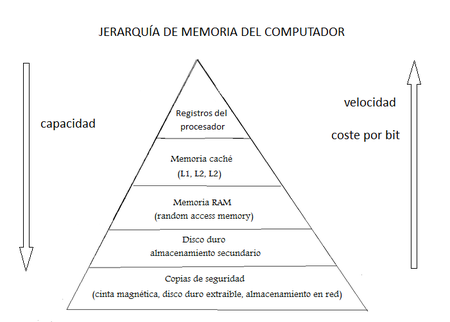
\includegraphics[scale=1]{images/jerarquia-de-memoria.png}
   \caption{Jerarquía de memoria}
   \label{speedup}
\end{figure}

En la jerarquía de memoria de un computador, los componentes más rápidos son también los que menos capacidad tienen y los más caros. Cuando un programa se ejecuta, dependiendo de la cantidad de almacenamiento que necesite, utilizan los distintos recursos de la jerarquía según cuánto necesite almacenar y según la disponibilidad de los mismos.

\vspace{4mm}
Rayo y Centella cuentan con las siguientes características:

\begin{center}
\begin{tabu} to 0.8\textwidth { | X[l] | X[l] | X[l] | X[l] | X[l] | }
 \hline
 \multicolumn{1}{|c|}{\bf Máquina} & \multicolumn{1}{|c|}{\bf L1} & \multicolumn{1}{|c|}{\bf L2} &  \multicolumn{1}{|c|}{\bf L3} &  \multicolumn{1}{|c|}{\bf RAM} \\
 \hline
 Rayo & \centering 1536KiB & \centering 6MiB & \centering 10MiB  & \centering 64GB\\
  \hline
   Centella &  \centering 576KiB & \centering 12MiB & \centering 12MiB & \centering 64GB \\
 \hline
\end{tabu}
\end{center}

En todas las gráficas generadas se obtienen una serie de resultados en común.

\begin{itemize}
 \item  En las gráficas de tiempo de ejecución, se puede observar que Centella realiza los cálculos más rápido que Rayo. Sin embargo, cuanto más aumenta el número de procesadores, ambas máquinas tienden a tener un tiempo de ejecución similar.
 \item  En las gráficas de la aceleración, la eficiencia, la utilización, la redundancia y la calidad del paralelismo, Rayo aparece generalmente por encima de Centella. Esto no significa que Rayo sea más potente ni más rápido, sino que Rayo se ve mucho más beneficiado de la ejecución paralela que Centella.
 \item Tanto para Rayo como para Centella ocurre speedup superlineal en la mayoría de algoritmos. Esto es así porque, tras utilizar un número determinado de procesadores, el tamaño del problema cabe en caché, que implica evitar el acceso a memoria RAM y, por tanto, acelerar muchísimo más los cálculos.
\end{itemize}

Los tamaños de problema para cada algoritmo son:

\begin{center}
\begin{tabular}{|l|l|l|l|l|}
\hline
Algoritmo & \multicolumn{4}{c|}{Tamaño de problema C} \\ \hline
IS        & \multicolumn{4}{l|}{$ 2^{27} $ claves con valor máximo de $ 2^{23} $}     \\ \hline
EP        & \multicolumn{4}{l|}{$ 2^{32} $ pares de números aleatorios}                   \\ \hline
CG        & \multicolumn{4}{l|}{150000 filas, 75 iteraciones, 15 no ceros}                   \\ \hline
MG        & \multicolumn{4}{l|}{Matriz 512 x 512 x 512, 20 iteraciones}                   \\ \hline
FT        & \multicolumn{4}{l|}{Matriz 512 x 512 x 512, 20 iteraciones}                   \\ \hline
BT        & \multicolumn{4}{l|}{Matriz 162 x 162 x 162, 200 iteraciones}                   \\ \hline
SP        & \multicolumn{4}{l|}{Matriz 162 x 162 x 162, 400 iteraciones}                   \\ \hline
LU        & \multicolumn{4}{l|}{Matriz 480 x 320 x 28, 0.8GB de memoria necesaria}                   \\ \hline
\end{tabular}
\end{center}

De todos los algoritmos, el que menos tiempo tardó en ejecutarse de media fue el de IS (Figura \ref{is:tiempo} y el que más el algoritmo de BT, matrices tridiagonales en bloque (Figura \ref{bt:tiempo}).

\vspace{2mm}

Una de las gráficas que llama más la atención es la de la Calidad del Paralelismo (Figura \ref{cg:calidad}), especialmente Centella. En este caso, Centella presenta un buen speed up (Figura \ref{cg:speedup}) y una buena eficiencia (Figura \ref{cg:eficiencia}). Sin embargo, la redundancia es muy alta (Figura \ref{cg:redundancia}, por lo que la calidad del paralelismo es mala.

\newpage

\subsection{Gráficas IS}

\begin{center}
 \centering
 \begin{minipage}[b]{.49\textwidth}
  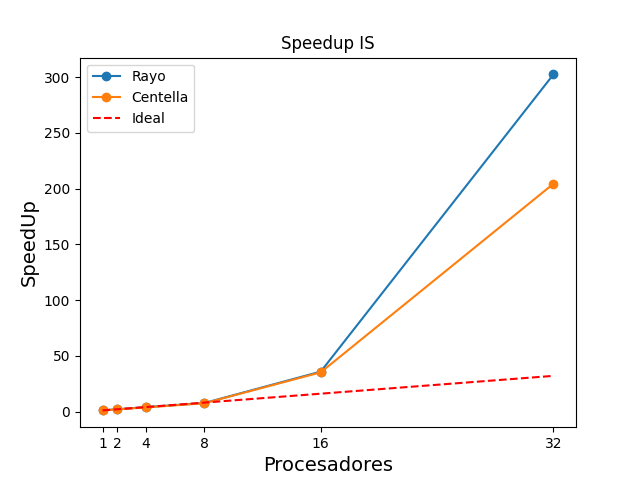
\includegraphics[width=1\linewidth]{plots/speed-up-is.png}
  \captionof{figure}{Speedup IS}
  \label{is:speedup}
 \end{minipage}
% \qquad
 \begin{minipage}[b]{.49\textwidth}
  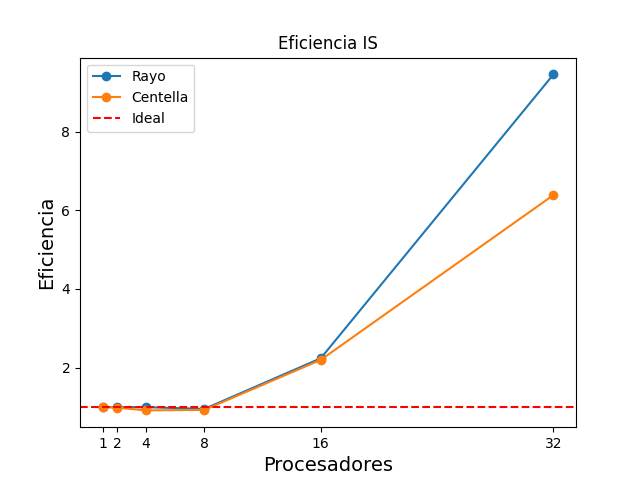
\includegraphics[width=1\linewidth]{plots/efficiency-is.png}
  \captionof{figure}{Eficiencia IS}
 \end{minipage}
\end{center}

\begin{center}
 \centering
  \begin{minipage}[b]{.49\textwidth}
  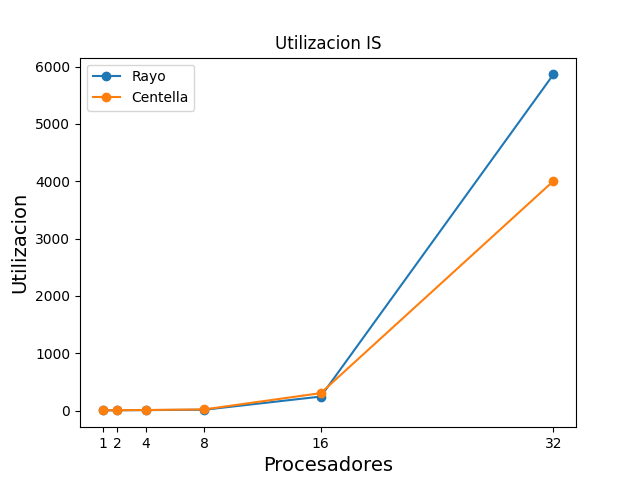
\includegraphics[width=1\linewidth]{plots/utilizacion-is.png}
  \captionof{figure}{Utilización IS}
 \end{minipage}
% \qquad
 \begin{minipage}[b]{.49\textwidth}
  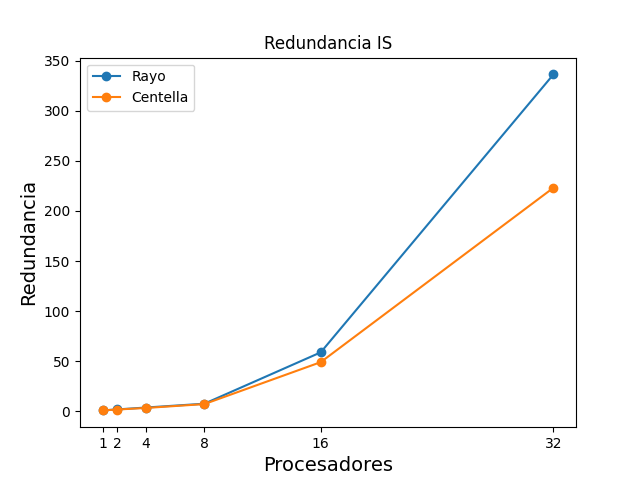
\includegraphics[width=1\linewidth]{plots/redundancy-is.png}
  \captionof{figure}{Redundancia IS}
 \end{minipage}
\end{center}

\begin{center}
 \centering
 \begin{minipage}[b]{.49\textwidth}
  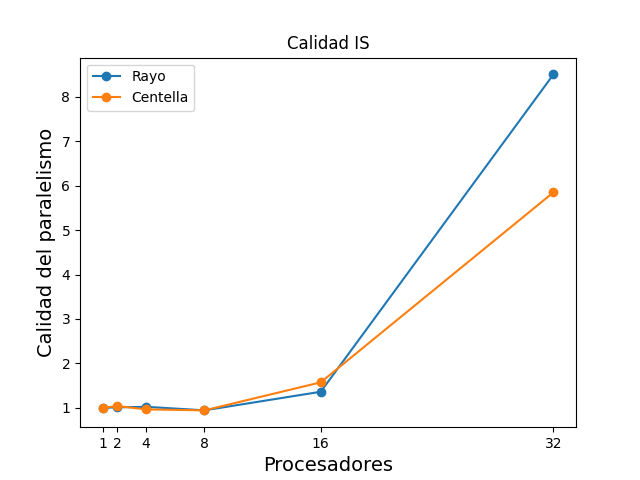
\includegraphics[width=1\linewidth]{plots/calidad-is.png}
  \captionof{figure}{Calidad Paralelismo IS}
 \end{minipage}
   % \qquad
 \begin{minipage}[b]{.49\textwidth}
  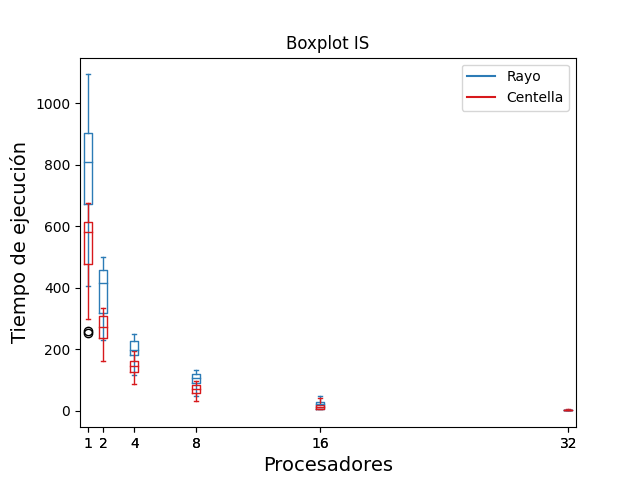
\includegraphics[width=1\linewidth]{plots/boxplot-is.png}
  \captionof{figure}{Tiempo Ejecución IS}
  \label{is:tiempo}
 \end{minipage}
\end{center}

\newpage

\subsection{Gráficas EP}

\begin{center}
 \centering
 \begin{minipage}[b]{.49\textwidth}
  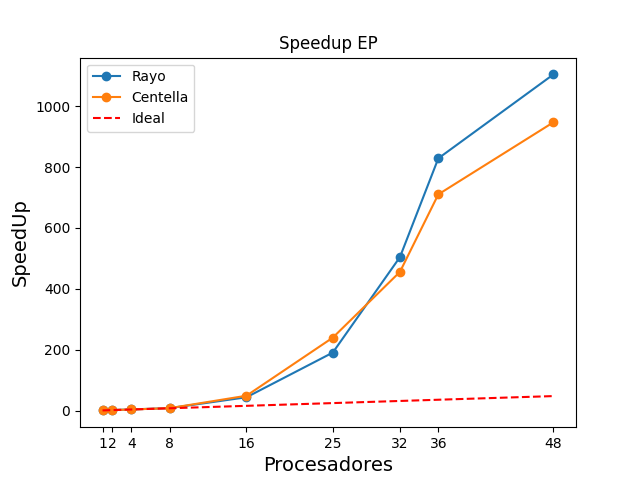
\includegraphics[width=1\linewidth]{plots/speed-up-ep.png}
  \captionof{figure}{Speedup EP}
  \label{ep:speedup}
 \end{minipage}
% \qquad
 \begin{minipage}[b]{.49\textwidth}
  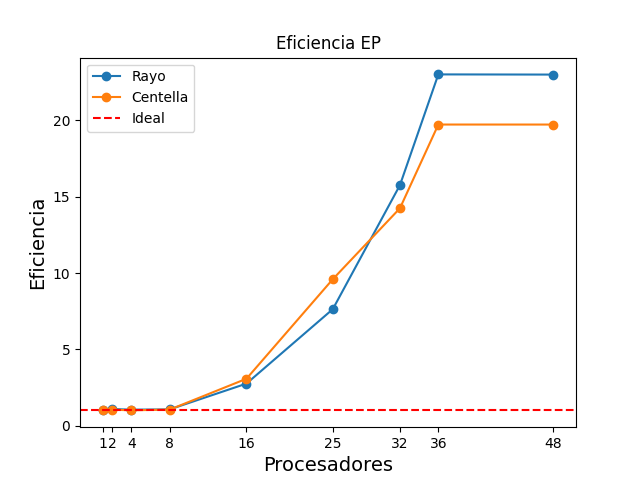
\includegraphics[width=1\linewidth]{plots/efficiency-ep.png}
  \captionof{figure}{Eficiencia EP}
 \end{minipage}
\end{center}

\begin{center}
 \centering
  \begin{minipage}[b]{.49\textwidth}
  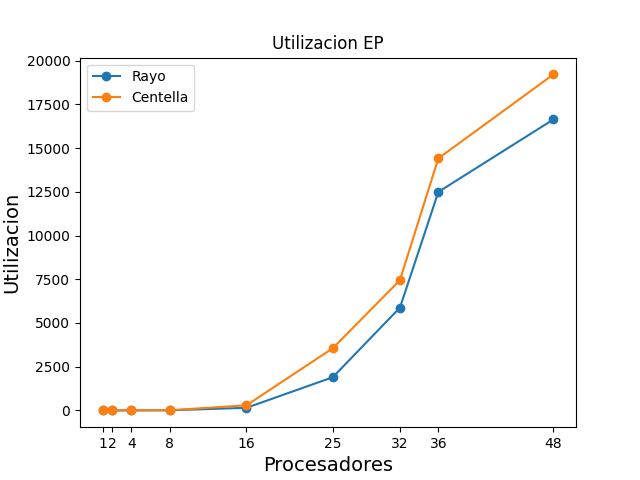
\includegraphics[width=1\linewidth]{plots/utilizacion-ep.png}
  \captionof{figure}{Utilización EP}
 \end{minipage}
% \qquad
 \begin{minipage}[b]{.49\textwidth}
  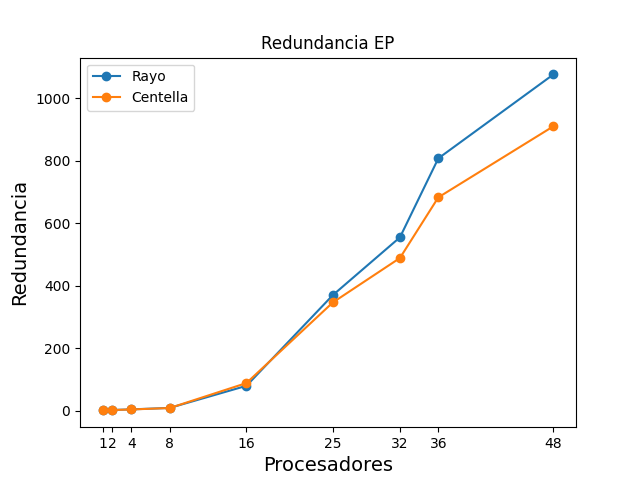
\includegraphics[width=1\linewidth]{plots/redundancy-ep.png}
  \captionof{figure}{Redundancia EP}
 \end{minipage}
\end{center}

\begin{center}
 \centering
 \begin{minipage}[b]{.49\textwidth}
  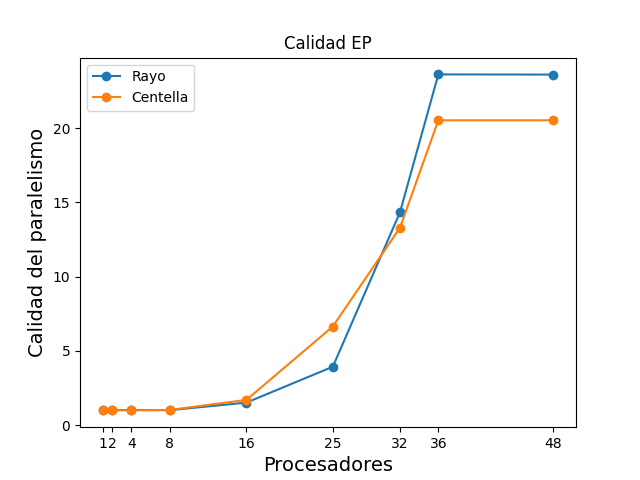
\includegraphics[width=1\linewidth]{plots/calidad-ep.png}
  \captionof{figure}{Calidad Paralelismo EP}
 \end{minipage}
  % \qquad
 \begin{minipage}[b]{.49\textwidth}
  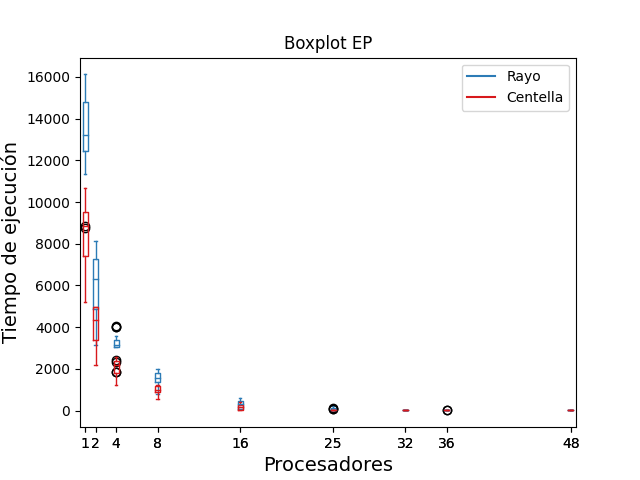
\includegraphics[width=1\linewidth]{plots/boxplot-ep.png}
  \captionof{figure}{Tiempo Ejecución EP}
 \end{minipage}
\end{center}

\newpage

\subsection{Gráficas CG}

\begin{center}
 \centering
 \begin{minipage}[b]{.49\textwidth}
  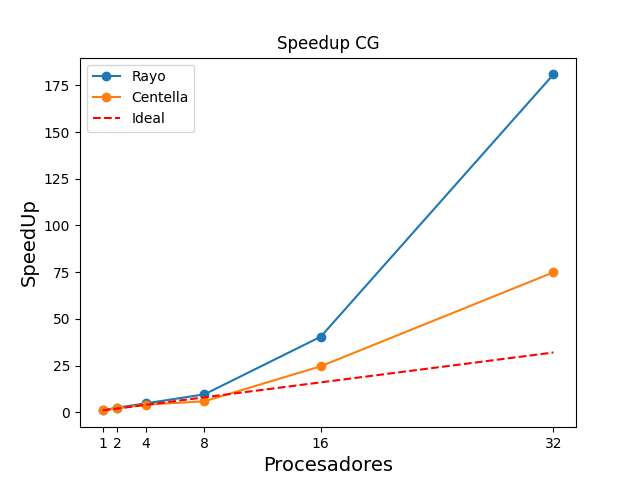
\includegraphics[width=1\linewidth]{plots/speed-up-cg.png}
  \label{cg:speedup}
  \captionof{figure}{Speedup CG}
 \end{minipage}
% \qquad
 \begin{minipage}[b]{.49\textwidth}
  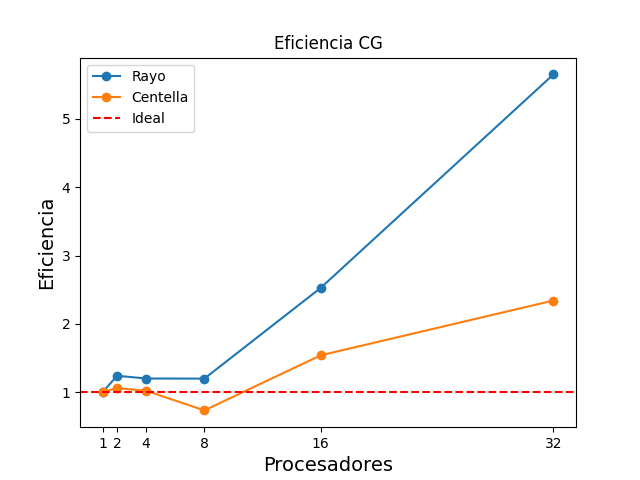
\includegraphics[width=1\linewidth]{plots/efficiency-cg.png}
  \captionof{figure}{Eficiencia CG}
    \label{cg:eficiencia}
 \end{minipage}
\end{center}

\begin{center}
 \centering
  \begin{minipage}[b]{.49\textwidth}
  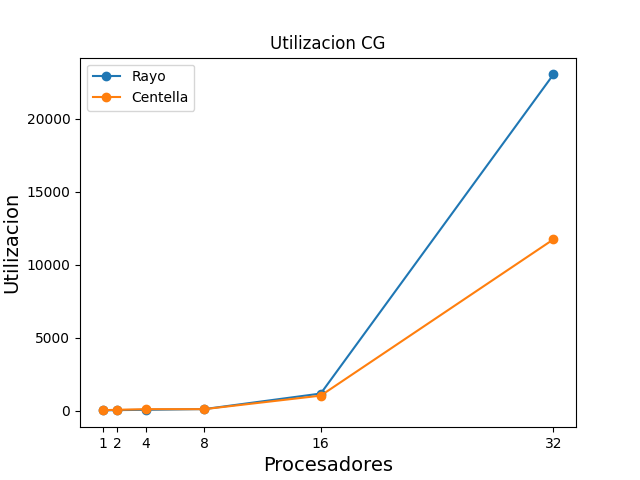
\includegraphics[width=1\linewidth]{plots/utilizacion-cg.png}
  \captionof{figure}{Utilización CG}
 \end{minipage}
% \qquad
 \begin{minipage}[b]{.49\textwidth}
  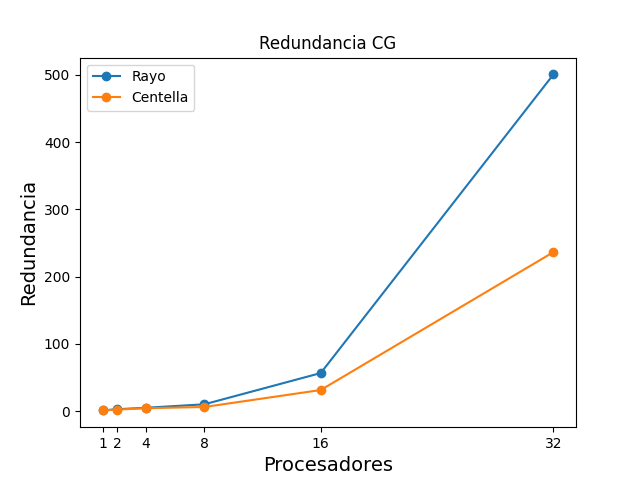
\includegraphics[width=1\linewidth]{plots/redundancy-cg.png}
  \captionof{figure}{Redundancia CG}
    \label{cg:redundancia}
 \end{minipage}
\end{center}

\begin{center}
 \centering
 \begin{minipage}[b]{.49\textwidth}
  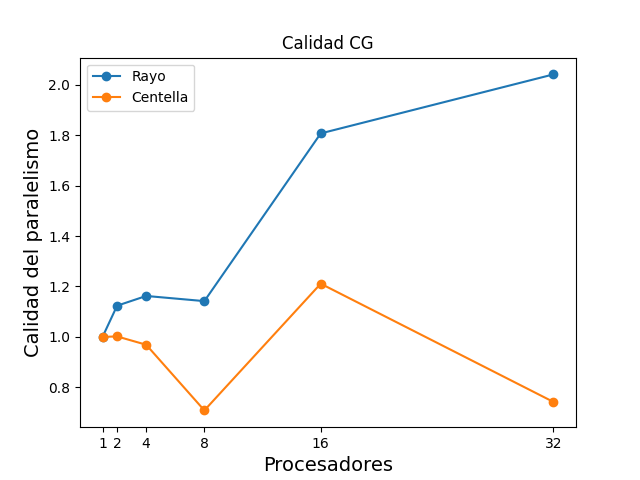
\includegraphics[width=1\linewidth]{plots/calidad-cg.png}
  \captionof{figure}{Calidad Paralelismo CG}
    \label{cg:calidad}
 \end{minipage}
  % \qquad
 \begin{minipage}[b]{.49\textwidth}
  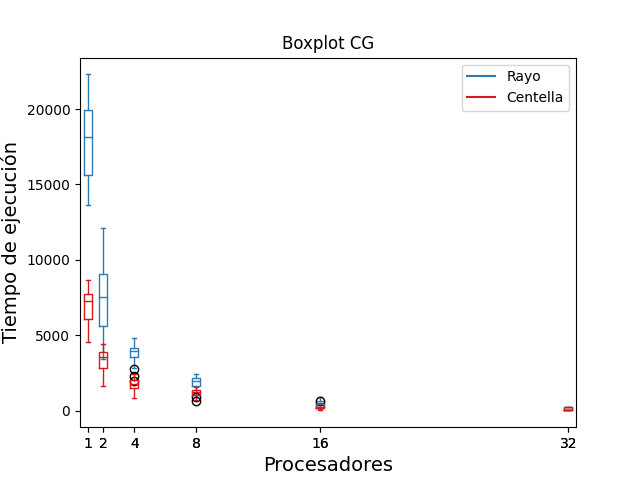
\includegraphics[width=1\linewidth]{plots/boxplot-cg.png}
    \label{cg:tiempo}
  \captionof{figure}{Tiempo Ejecución CG}
 \end{minipage}
\end{center}

\newpage

\subsection{Gráficas MG}

\begin{center}
 \centering
 \begin{minipage}[b]{.49\textwidth}
  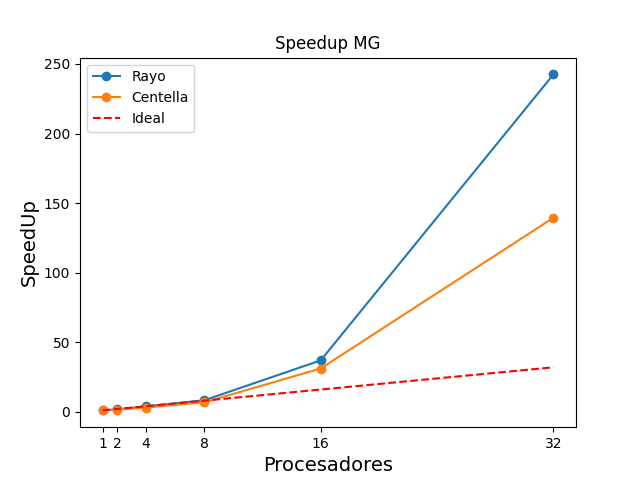
\includegraphics[width=1\linewidth]{plots/speed-up-mg.png}
  \captionof{figure}{Speedup MG}
 \end{minipage}
% \qquad
 \begin{minipage}[b]{.49\textwidth}
  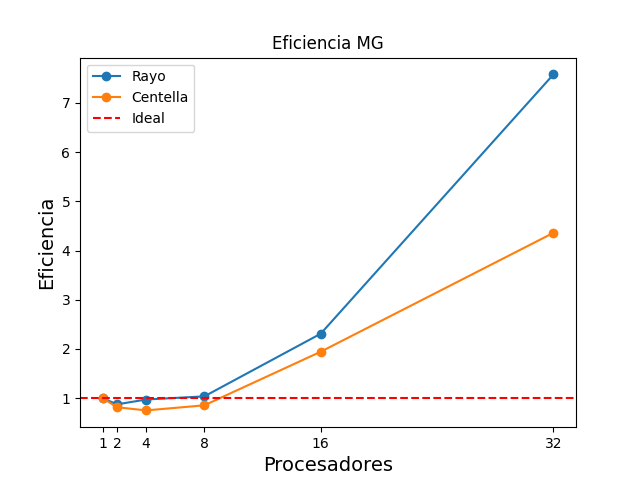
\includegraphics[width=1\linewidth]{plots/efficiency-mg.png}
  \captionof{figure}{Eficiencia MG}
 \end{minipage}
\end{center}

\begin{center}
 \centering
  \begin{minipage}[b]{.49\textwidth}
  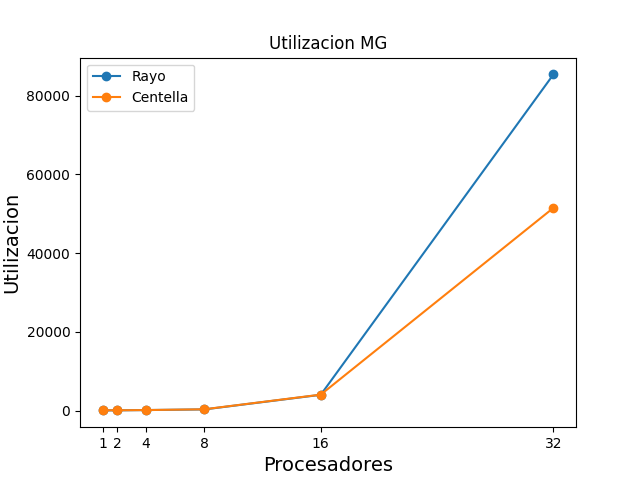
\includegraphics[width=1\linewidth]{plots/utilizacion-mg.png}
  \captionof{figure}{Utilización MG}
 \end{minipage}
% \qquad
 \begin{minipage}[b]{.49\textwidth}
  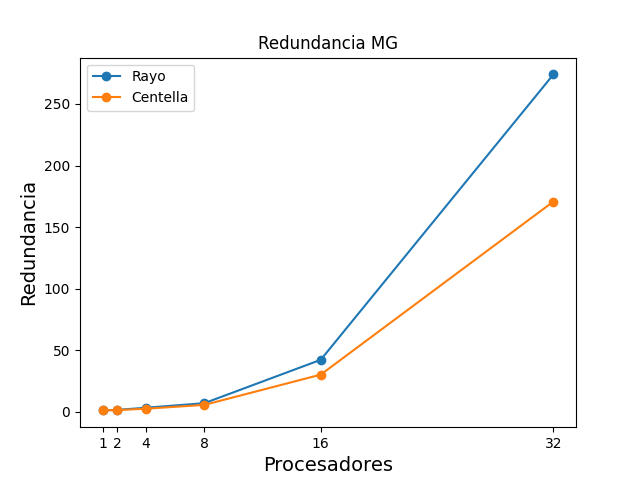
\includegraphics[width=1\linewidth]{plots/redundancy-mg.png}
  \captionof{figure}{Redundancia MG}
 \end{minipage}
\end{center}

\begin{center}
 \centering
 \begin{minipage}[b]{.49\textwidth}
  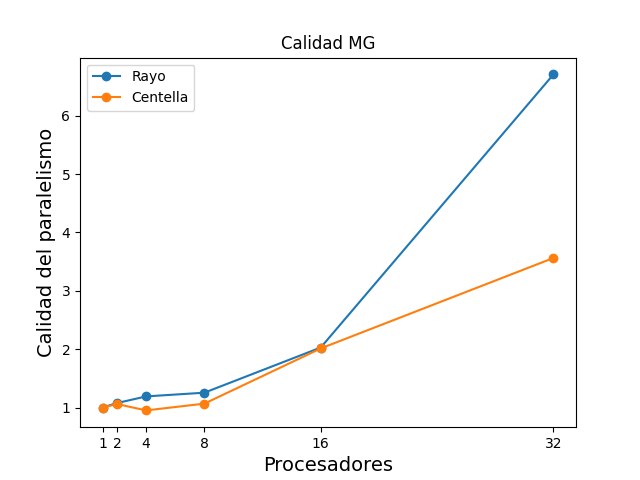
\includegraphics[width=1\linewidth]{plots/calidad-mg.png}
  \captionof{figure}{Calidad Paralelismo MG}
 \end{minipage}
  % \qquad
 \begin{minipage}[b]{.49\textwidth}
  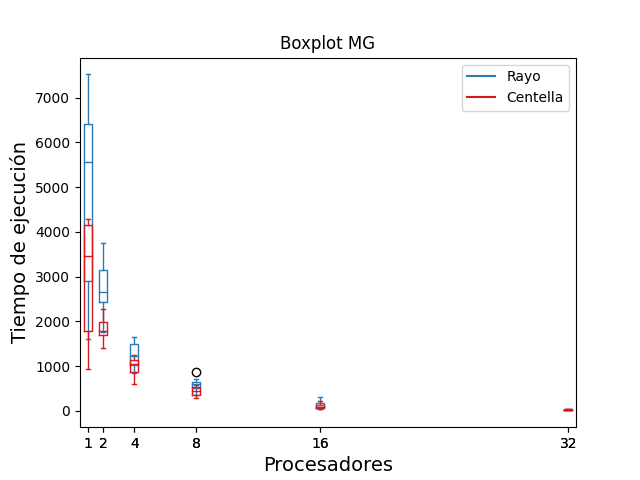
\includegraphics[width=1\linewidth]{plots/boxplot-mg.png}
  \captionof{figure}{Tiempo Ejecución MG}
 \end{minipage}
\end{center}

\newpage

\subsection{Gráficas FT}

\begin{center}
 \centering
 \begin{minipage}[b]{.49\textwidth}
  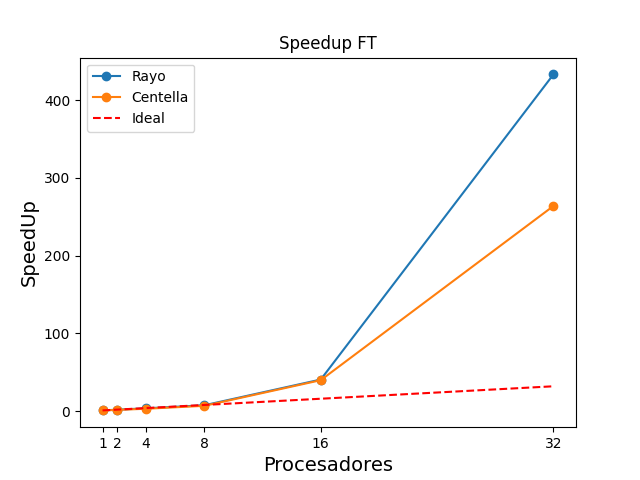
\includegraphics[width=1\linewidth]{plots/speed-up-ft.png}
  \captionof{figure}{Speedup FT}
  \label{ft:speedup}
 \end{minipage}
% \qquad
 \begin{minipage}[b]{.49\textwidth}
  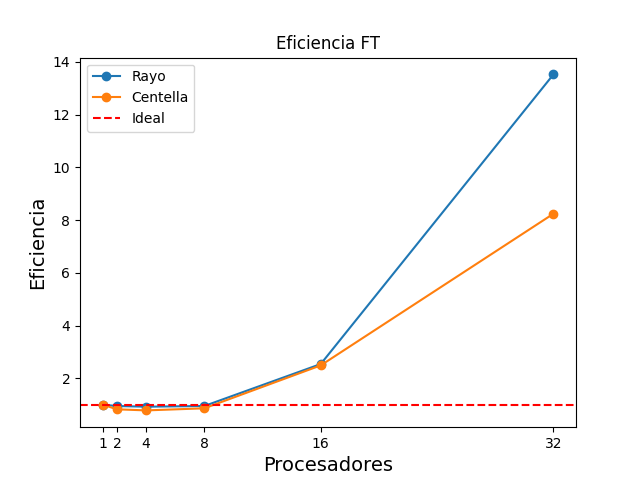
\includegraphics[width=1\linewidth]{plots/efficiency-ft.png}
  \captionof{figure}{Eficiencia FT}
 \end{minipage}
\end{center}

\begin{center}
 \centering
  \begin{minipage}[b]{.49\textwidth}
  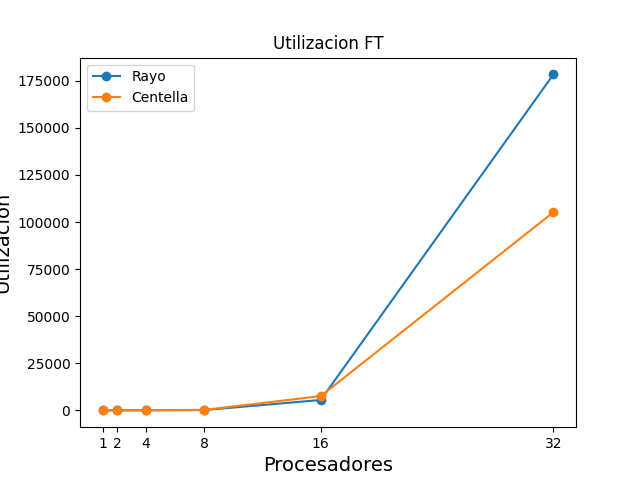
\includegraphics[width=1\linewidth]{plots/utilizacion-ft.png}
  \captionof{figure}{Utilización FT}
 \end{minipage}
% \qquad
 \begin{minipage}[b]{.49\textwidth}
  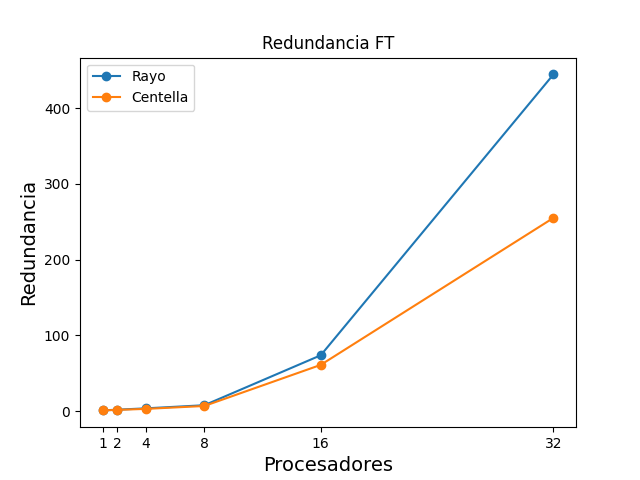
\includegraphics[width=1\linewidth]{plots/redundancy-ft.png}
  \captionof{figure}{Redundancia FT}
 \end{minipage}
\end{center}

\begin{center}
 \centering
 \begin{minipage}[b]{.49\textwidth}
  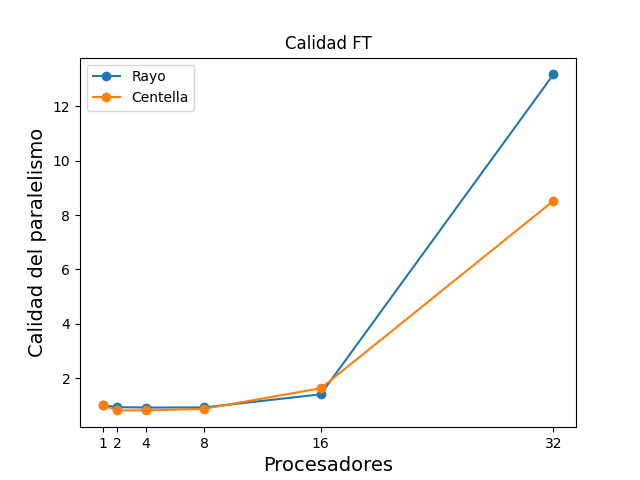
\includegraphics[width=1\linewidth]{plots/calidad-ft.png}
  \captionof{figure}{Calidad Paralelismo FT}
 \end{minipage}
  % \qquad
 \begin{minipage}[b]{.49\textwidth}
  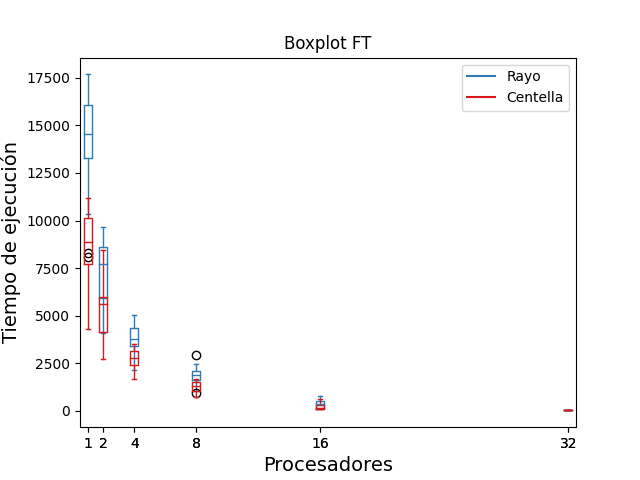
\includegraphics[width=1\linewidth]{plots/boxplot-ft.png}
  \captionof{figure}{Tiempo Ejecución FT}
 \end{minipage}
\end{center}

\newpage

\subsection{Gráficas BT}

\begin{center}
 \centering
 \begin{minipage}[b]{.49\textwidth}
  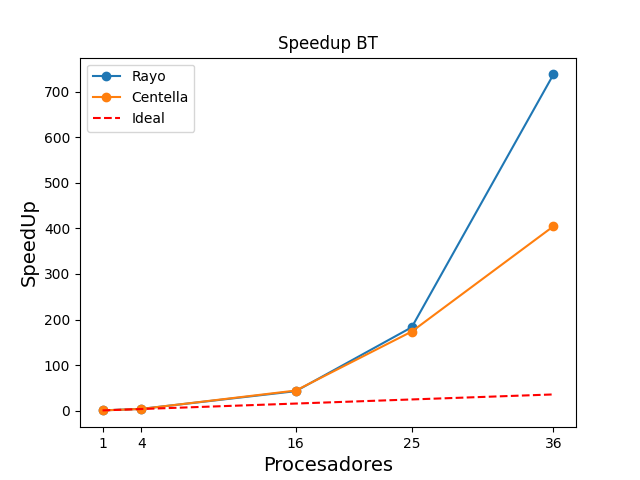
\includegraphics[width=1\linewidth]{plots/speed-up-bt.png}
  \captionof{figure}{Speedup BT}
 \end{minipage}
% \qquad
 \begin{minipage}[b]{.49\textwidth}
  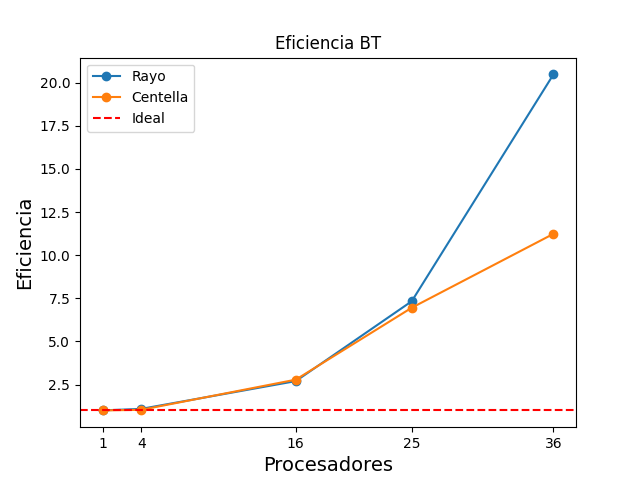
\includegraphics[width=1\linewidth]{plots/efficiency-bt.png}
  \captionof{figure}{Eficiencia BT}
 \end{minipage}
\end{center}

\begin{center}
 \centering
  \begin{minipage}[b]{.49\textwidth}
  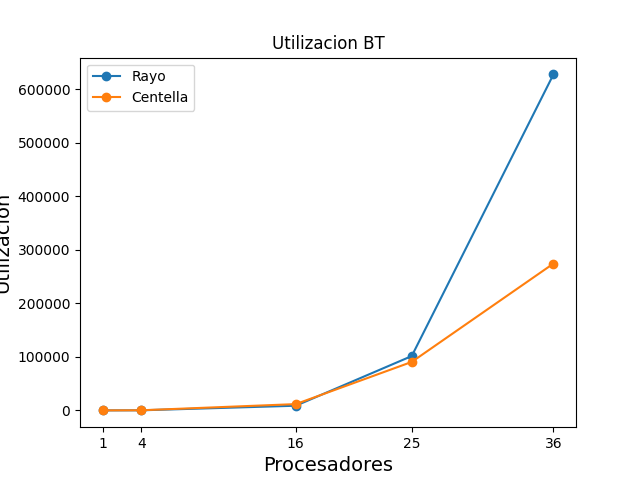
\includegraphics[width=1\linewidth]{plots/utilizacion-bt.png}
  \captionof{figure}{Utilización BT}
 \end{minipage}
% \qquad
 \begin{minipage}[b]{.49\textwidth}
  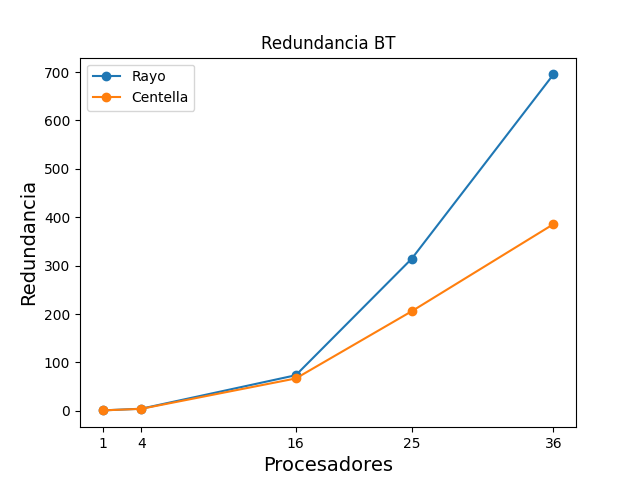
\includegraphics[width=1\linewidth]{plots/redundancy-bt.png}
  \captionof{figure}{Redundancia BT}
 \end{minipage}
\end{center}

\begin{center}
 \centering
 \begin{minipage}[b]{.49\textwidth}
  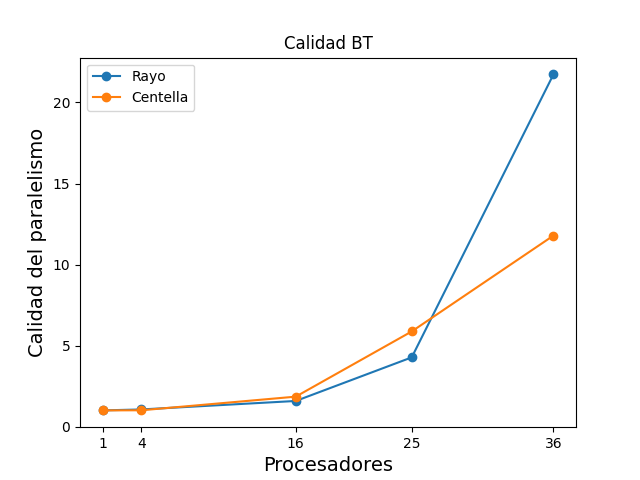
\includegraphics[width=1\linewidth]{plots/calidad-bt.png}
  \captionof{figure}{Calidad Paralelismo BT}
 \end{minipage}
  % \qquad
 \begin{minipage}[b]{.49\textwidth}
  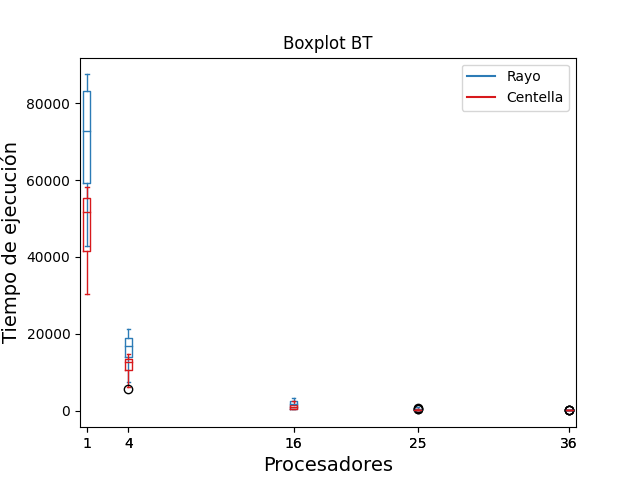
\includegraphics[width=1\linewidth]{plots/boxplot-bt.png}
  \label{bt:tiempo}
  \captionof{figure}{Tiempo Ejecución BT}
 \end{minipage}
\end{center}

\newpage

\subsection{Gráficas SP}

\begin{center}
 \centering
 \begin{minipage}[b]{.49\textwidth}
  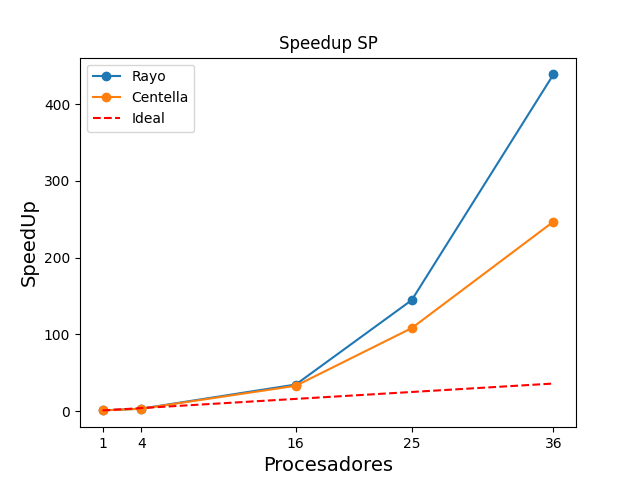
\includegraphics[width=1\linewidth]{plots/speed-up-sp.png}
  \captionof{figure}{Speedup SP}
 \end{minipage}
% \qquad
 \begin{minipage}[b]{.49\textwidth}
  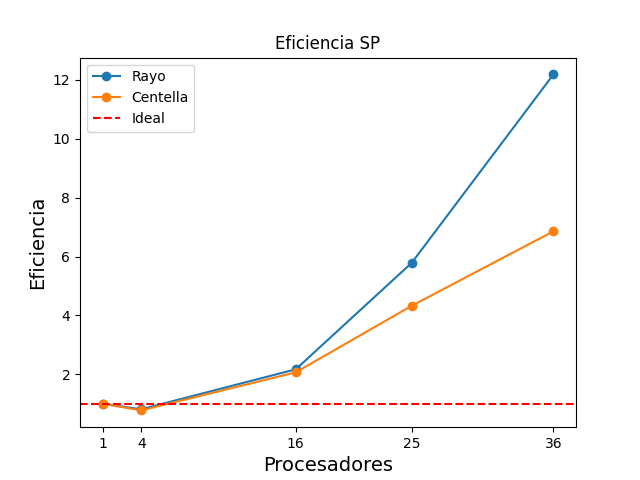
\includegraphics[width=1\linewidth]{plots/efficiency-sp.png}
  \captionof{figure}{Eficiencia SP}
 \end{minipage}
\end{center}

\begin{center}
 \centering
  \begin{minipage}[b]{.49\textwidth}
  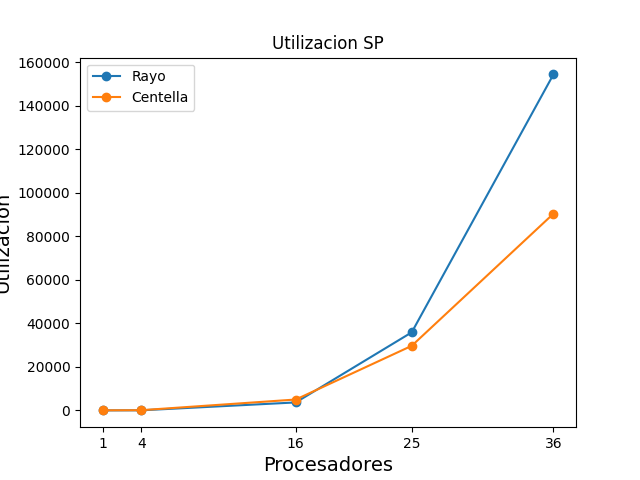
\includegraphics[width=1\linewidth]{plots/utilizacion-sp.png}
  \captionof{figure}{Utilización SP}
 \end{minipage}
% \qquad
 \begin{minipage}[b]{.49\textwidth}
  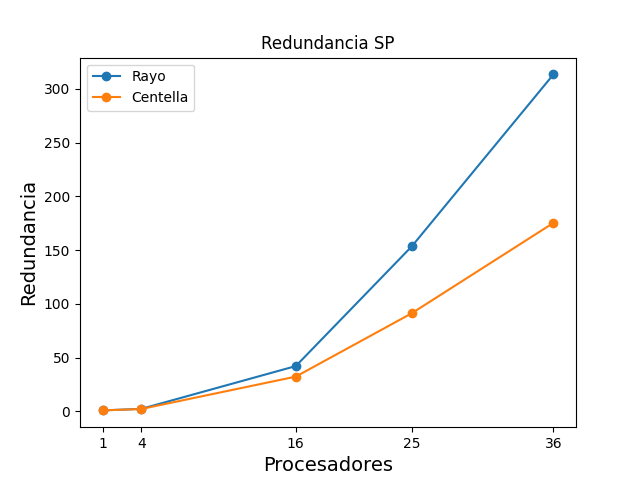
\includegraphics[width=1\linewidth]{plots/redundancy-sp.png}
  \captionof{figure}{Redundancia SP}
 \end{minipage}
\end{center}

\begin{center}
 \centering
 \begin{minipage}[b]{.49\textwidth}
  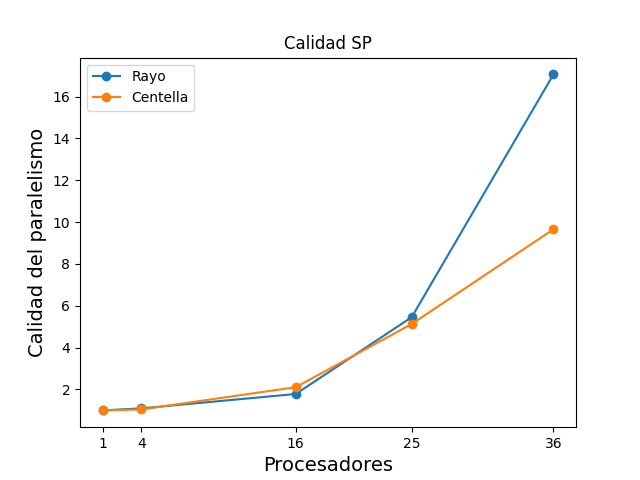
\includegraphics[width=1\linewidth]{plots/calidad-sp.png}
  \captionof{figure}{Calidad Paralelismo SP}
 \end{minipage}
  % \qquad
 \begin{minipage}[b]{.49\textwidth}
  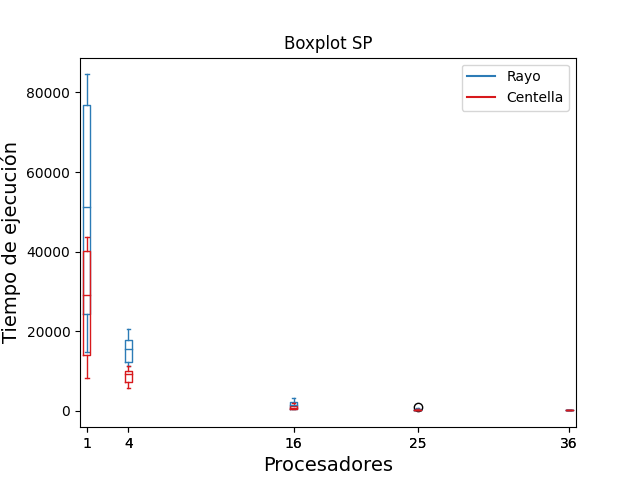
\includegraphics[width=1\linewidth]{plots/boxplot-sp.png}
  \captionof{figure}{Tiempo Ejecución SP}
 \end{minipage}
\end{center}

\newpage

\subsection{Gráficas LU}

\begin{center}
 \centering
 \begin{minipage}[b]{.49\textwidth}
  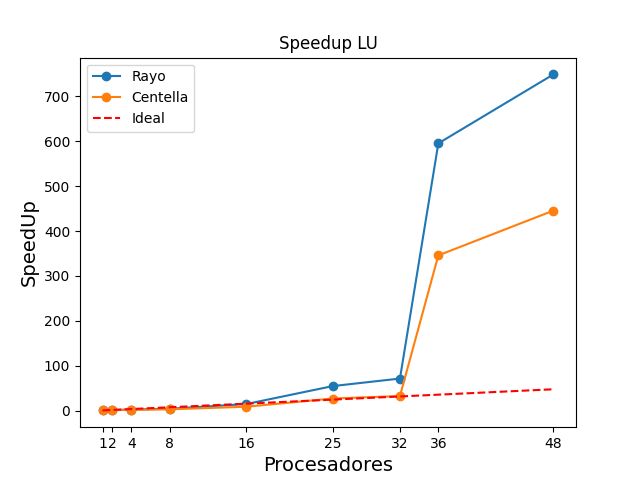
\includegraphics[width=1\linewidth]{plots/speed-up-lu.png}
  \captionof{figure}{Speedup LU}
 \end{minipage}
% \qquad
 \begin{minipage}[b]{.49\textwidth}
  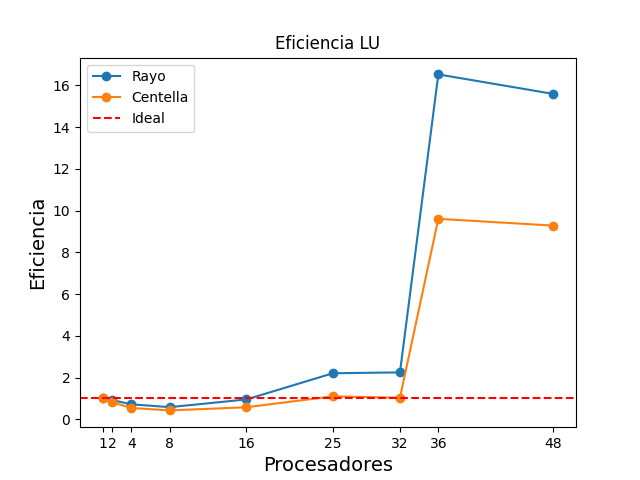
\includegraphics[width=1\linewidth]{plots/efficiency-lu.png}
  \captionof{figure}{Eficiencia LU}
 \end{minipage}
\end{center}

\begin{center}
 \centering
  \begin{minipage}[b]{.49\textwidth}
  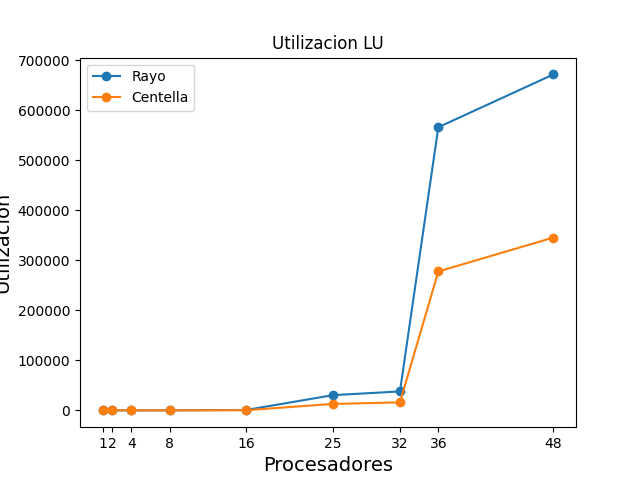
\includegraphics[width=1\linewidth]{plots/utilizacion-lu.png}
  \captionof{figure}{Utilización LU}
 \end{minipage}
% \qquad
 \begin{minipage}[b]{.49\textwidth}
  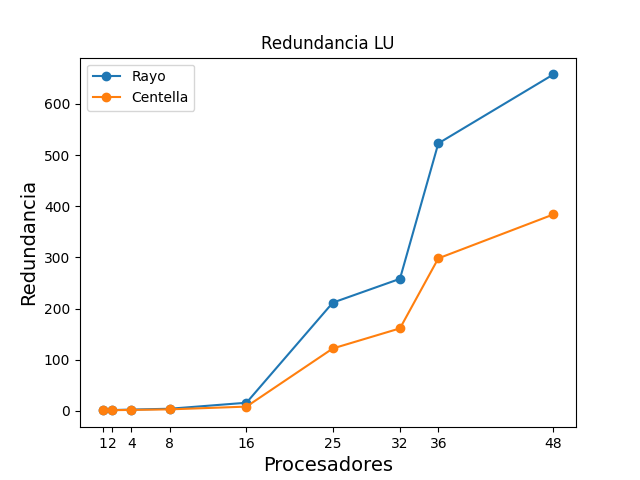
\includegraphics[width=1\linewidth]{plots/redundancy-lu.png}
  \captionof{figure}{Redundancia LU}
 \end{minipage}
\end{center}

\begin{center}
 \centering
 \begin{minipage}[b]{.49\textwidth}
  \includegraphics[width=1\linewidth]{plots/calidad-LU.png}
  \captionof{figure}{Calidad Paralelismo LU}
 \end{minipage}
 % \qquad
 \begin{minipage}[b]{.49\textwidth}
  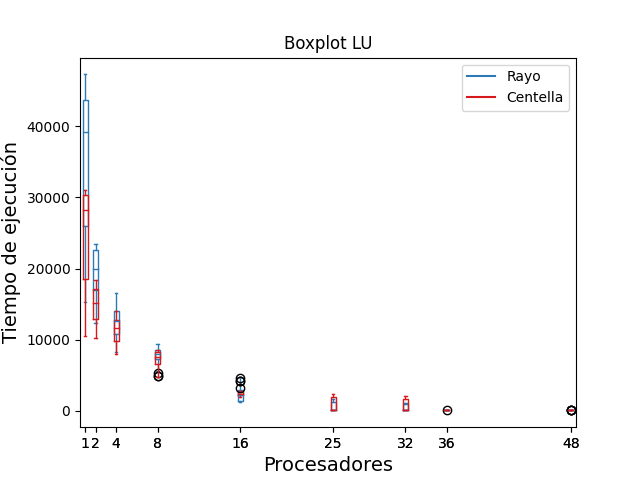
\includegraphics[width=1\linewidth]{plots/boxplot-lu.png}
  \captionof{figure}{Tiempo Ejecución LU}
 \end{minipage}
\end{center}
